\documentclass[11pt]{article}
\usepackage[a4paper,margin=1in]{geometry}
\usepackage{amsmath,amssymb}
\usepackage{xcolor}
\usepackage{booktabs}
\usepackage{tikz}
\usepackage{parskip}
\usepackage{titlesec}
\usetikzlibrary{positioning, arrows.meta, fit}

\titleformat{\section}{\large\bfseries}{\thesection}{0.6em}{}

\title{Velocity vs.\ angle: what the network encodes\\
\large Hulse Model A path-integration RNN}
\author{Internal note, connectome-gnn project}
\date{2026-05-13}

\begin{document}
\maketitle

\section*{The headline}

The network's recurrent state $h(t) \in \mathbb{R}^{152}$ encodes \textbf{one
quantity}: \emph{head direction} $\hat\theta_{\text{hd}}(t)$ --- an angle ---
through the position of an activity bump on the EPG ring.

\textbf{Velocity is not part of the state.} $\omega(t)$ is an external input
delivered every timestep through $W^{\mathrm{in}}_{:,0}$ that \emph{rotates}
the bump. The "integrate velocity to get heading" relationship,
\begin{equation}
\hat\theta_{\text{hd}}(t) \;=\; \theta_0 \;+\; \int_0^{t}\hat\omega(s)\,ds,
\end{equation}
is the \emph{function} the network has to learn, not a state variable it
keeps track of explicitly.

\section*{Input / output / state}

\begin{center}
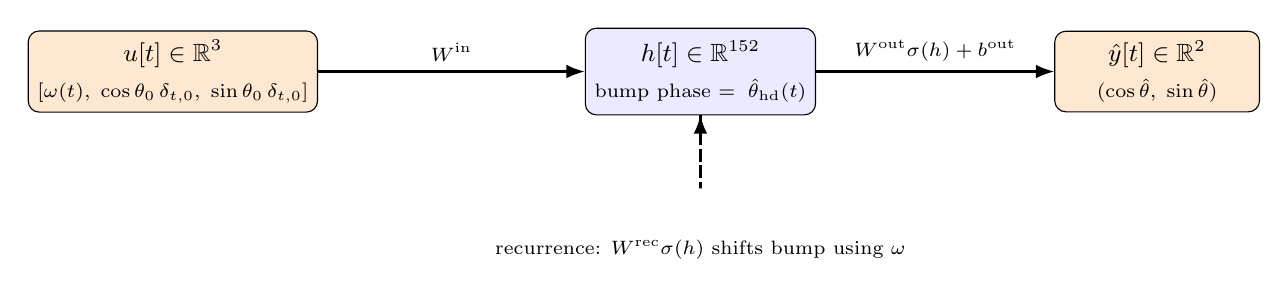
\begin{tikzpicture}[
  every node/.style={font=\small},
  blk/.style={draw, rounded corners, minimum width=2.4cm, minimum height=1.1cm,
              align=center, fill=blue!8},
  inp/.style={draw, rounded corners, minimum width=2.6cm, minimum height=0.9cm,
              align=center, fill=orange!18, font=\small},
  oblk/.style={inp},
  arr/.style={-Latex, thick}
]
\node[inp] (u) at (0, 0)
   {$u[t]\in\mathbb{R}^{3}$\\[2pt]
    {\scriptsize $[\omega(t),\;\cos\theta_0\,\delta_{t,0},\;\sin\theta_0\,\delta_{t,0}]$}};
\node[blk] (h) at (6.7, 0)
   {$h[t]\in\mathbb{R}^{152}$\\[2pt]
    {\scriptsize bump phase $=\;\hat\theta_{\text{hd}}(t)$}};
\node[oblk] (y) at (12.5, 0)
   {$\hat y[t]\in\mathbb{R}^{2}$\\[2pt]
    {\scriptsize $(\cos\hat\theta,\;\sin\hat\theta)$}};
\draw[arr] (u) -- node[above, font=\scriptsize]{$W^{\mathrm{in}}$} (h);
\draw[arr] (h) -- node[above, font=\scriptsize]{$W^{\mathrm{out}}\sigma(h)+b^{\mathrm{out}}$} (y);
\draw[arr, dashed] (h.south) .. controls +(0,-1.2) and +(0,-1.2) .. (h.south)
  node[below, font=\scriptsize, midway, yshift=-0.55cm]
  {recurrence: $W^{\mathrm{rec}}\sigma(h)$ shifts bump using $\omega$};
\end{tikzpicture}
\end{center}

\textbf{Three ways velocity makes the bump move.} The network has no explicit
velocity-modulated connectivity matrix (unlike Noorman's $W^{\mathrm{cw}}/W^{\mathrm{ccw}}$).
Instead, it learns to use the input pathway:
\begin{enumerate}
\item $\omega(t)$ excites the PEN cells (which our W$_\mathrm{in}$ inspection
showed receive the largest $W^{\mathrm{in}}_{:,0}$ weights).
\item PEN cells push the EPG bump through the connectome's PEN $\to$ EPG
asymmetric pathway.
\item The bump slides to a new position; the readout reports the new angle.
\end{enumerate}

\section*{Three components of "integration"}

If you treat the network as a black-box integrator, three things have to be
right simultaneously:

\begin{center}\small
\begin{tabular}{lll}
\toprule
\textbf{Component} & \textbf{Lives in} & \textbf{Failure mode} \\
\midrule
Bump stability ($\omega=0$ $\Rightarrow$ bump holds) & $W^{\mathrm{rec}}$, $b$ & bump drifts or decays at rest \\
Velocity gain ($\omega$ $\Rightarrow$ right rotation rate) & $W^{\mathrm{in}}_{:,0}\times$ PEN$\to$EPG pathway & constant-rate drift \\
Initial alignment ($\theta_0$ $\Rightarrow$ right bump phase) & $W^{\mathrm{in}}_{:,1:3}$ + transient at $t{=}0$ & wrong starting angle \\
\bottomrule
\end{tabular}
\end{center}

The MSE loss is on the readout angle, so all three are optimised jointly.
The Hulse "hidden symmetry" finding is that there are directions in
parameter space along which these components can drift \emph{without the
loss noticing} --- e.g.\ the velocity gain and the bump width can co-vary
in a way that keeps short-horizon integration accurate.

\section*{Two flavours of "drift"}

Constant phase offset $\hat\theta = \theta + \varepsilon_0$ is the ring
attractor's free SO(2) mode --- harmless. Constant rate
$\hat\theta = \theta + \varepsilon_0 + \varepsilon_1 t$ is a velocity-gain
miscalibration --- measurable and harmless if small.
The dangerous one is the random-walk diffusion that scales as $\sqrt{t}$ ---
the hidden-symmetry drift Hulse identifies.

\section*{Why this distinction matters for Phase B}

Phase B asks: given recorded activity (rate trajectories $\sigma(h(t))$),
can a GNN recover the connectivity matrix $W^{\mathrm{rec}}$? The answer is
\emph{only modulo the symmetry orbits}. Constant phase offsets and small
velocity-gain miscalibrations belong to the unidentifiable directions --- we
should evaluate recovery up to that equivalence, not against the bare
$W^{\mathrm{rec}}$ matrix entries.

\end{document}
